\documentclass[12pt, oneside]{article}
\usepackage[margin=1in]{geometry} 
\geometry{letterpaper}
\usepackage{graphicx}	
\usepackage{amssymb, amsmath}
\usepackage{natbib}
\usepackage{subfigure}
\usepackage{url}
\usepackage{fancyhdr}
\usepackage{lastpage}
\usepackage{fourier-orns}
\usepackage{tikz}

\usetikzlibrary{intersections, backgrounds, calc}

\definecolor{light}{RGB}{220, 188, 188}
\definecolor{mid}{RGB}{185, 124, 124}
\definecolor{dark}{RGB}{143, 39, 39}
\definecolor{highlight}{RGB}{0, 255, 0}
\definecolor{gray60}{gray}{0.6}
\definecolor{gray70}{gray}{0.7}
\definecolor{gray80}{gray}{0.8}
\definecolor{gray90}{gray}{0.9}
\definecolor{gray95}{gray}{0.95}

\graphicspath{{figures/}}

\pagestyle{fancy}
\fancyhf{}
\lfoot{
\includegraphics[width=8mm]{stan_logo.eps}}
\rfoot{\thepage \hspace{1pt} of \pageref{LastPage}}

\renewcommand{\headrulewidth}{0pt}
\renewcommand{\footrulewidth}{1pt}

\renewcommand\footrule{\hrulefill \raisebox{-15pt}[10pt][10pt]{
\includegraphics[width=6.5in]{line.eps}} \hrulefill}

\begin{document}
\thispagestyle{empty}

\begin{center}
\begin{tikzpicture}[scale=1, thick]
%\begin{tikzpicture}[scale=1, thick, show background rectangle]
 \node[] at (0, 0) {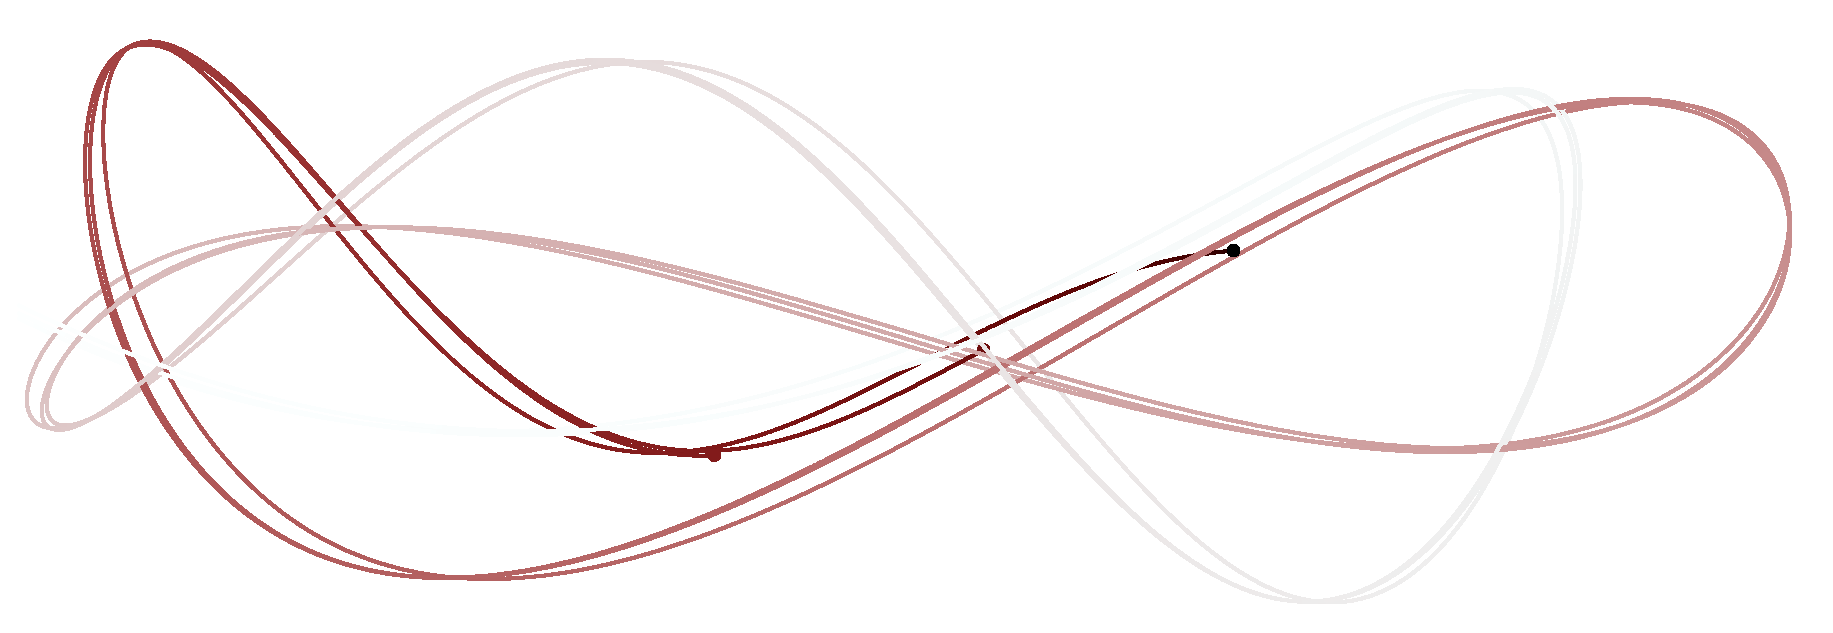
\includegraphics[width=16cm]{wide_ensemble.eps}};
 \node[] at (0, 2.5) {
\includegraphics[width=6cm]{stan_logo.eps}};
\end{tikzpicture}

\vspace{5mm}
\scalebox{10}{\fontsize{10pt}{0pt}\selectfont \textit{Stan}}
\vspace{10mm}

\end{center}

Fueled by technological and methodological advances, scientists,
engineers, and business analysts are collecting more and more 
complicated data.  To learn from that data, however, we have to build 
statistical models of the experiments from which the measurements
were made and then then identify the configurations of those models 
that are consistent with the measurements.  In particular, to accurately 
quantify our uncertainty we need to identify not just some consistent 
model configurations but \emph{all} consistent model configurations.
Fortunately, recent advances in statistical computing have revolutionized
our ability to build robust statistical analyses in these complex problems.  

Stan is a statistical library that facilitates general modeling, analysis, 
and prediction.  Users first specify their models with a probabilistic 
programming language from which they can generate inferences
using

\begin{itemize}
\item full Bayesian inference with scalable Hamiltonian Monte Carlo
\item approximate Bayesian inference with automatic variational inference 
\item penalized maximum likelihood estimation with optimization.
\end{itemize}

These inferences are built on top of a powerful C++ math library that provides 
differentiable probability functions and linear algebra.  Additional R packages 
provide expression-based linear modeling, posterior visualization, and model
validation.

\pagebreak

Stan has already had a very broad impact; thousands of people are using Stan 
to fit models, and scores of scientific papers have been written using Stan; a 
Google Scholar search for Stan's home page shows citations in clinical drug trials, 
general computational statistics, entomology, opthalmology, neurology, sociology 
and population dynamics, genomics, agriculture, psycholinguistics, molecular biology, 
population dynamics, materials engineering, botany, astrophysics, oceanography, 
election prediction, fisheries, cancer biology, public health and epidemiology, population 
ecology, collaborative filtering for recommender systems, climatology, educational 
testing, and natural language processing.

Because Stan is distributed through multiple channels that do not share detailed
statistics, estimating the total number of active users is subtle.  We can gauge the
growth of our community, however, by studying a subgroups such as those who
download Stan through RStudio (Figure \ref{fig:rstan_stats}).  The sustained growth
of this subcommunity indicates that the entire community is prospering.

\begin{figure}
\centering
\subfigure[] {\includegraphics[width=3.15in]{rstan_cum.eps} }
\subfigure[] {\includegraphics[width=3.15in]{rstan_diff.eps} }
\caption{Exact download statistics are limited, but we can gauge the overall
growth of the Stan community by looking at subgroups that do offer statistics,
such as users who employ Stan through RStudio.  The (a) cumulative and (b)
differential downloads indicate sustained growth of this subcommunity and,
hence, the entire Stan community.
}
\label{fig:rstan_stats}
\end{figure}

Stan is freedom-respecting, open-source software (new BSD core, some interfaces GPLv3)
that is associated with NumFOCUS, a 501(c)(3) nonprofit supporting open code and 
reproducible science.  All of Stan products have been released under the most generous 
open-source licenses possible. Stan?s licensing satisifies the goals listed in the solicitation for 
software sharing:

\begin{enumerate}
\item it is freely available to everyone, not just researchers;
\item it is licensed so that it may be freely extended, customized, and incorporated into 
         the maximal number of other tools;
\item the open-source licensing allows continuation of the project in the event of the original 
         developers not being willing or able to;
\item researchers are free to modify the official versions of the software released by the Stan 
         development team;
\item integration of user-provided code back into the core product for bug-fixes, examples, and 
         enhancements is carried out using GitHub pull requests with integration testing.
\end{enumerate}

\pagebreak

\section*{Testimonials}

\noindent Prof. Joseph A. Formaggio

\noindent Physics Department, Massachusetts Institute of Technology

\textit{
Stan has been an indispensable tool in the analysis of complex data by our group at MIT.  
I insist that all our incoming graduate students learn to use it when they join our group, 
knowing that it can be quite powerful in whatever analysis they will later undertake in their 
time here.  Our most recent paper, ``Violation of the Leggett-Garg Inequality in Neutrino 
Oscillations'' (Phys.Rev.Lett. 117 (2016), 050402) greatly benefited from having Stan as 
our analysis tool.}

\vspace{10mm}

\noindent Nathan Sanders

\noindent Senior Director of Quantitative Analytics, Legendary Entertainment

\noindent (Formerly Graduate Researcher, Harvard-Smithsonian Center for Astrophysics)


\textit{
I first encountered Stan while completing my PhD in
astrophysics right after it hit version 1.0.  It immediately had an
impact on my research.  Because the Stan modeling language is so
intuitive and the NUTS sampler is so robust, it became the first
modeling tool I reached for.  It allowed me to easily transition
classical models in my field from a maximum-likelihood to a full
Bayesian framework, and to innovate new and complex models while
focusing on scientific inferences rather than sampling algorithms and
execution efficiency.  My collaborators and I built a hierarchical
model for supernova light curves, thousands of data points
representing the brightness of exploding red supergiants at different
wavelengths as the explosions evolve over time, that enabled us to
directly model the population parameters of the progenitor stars of
these explosions while accounting for a variety of observational
biases like censoring, truncation, and selection effects.}

\textit{
Today, I use Stan as a primary mechanism for my work in industry.
It's a terrific tool for our data science team here because the Stan
language makes it straightforward to share human-readable models that
can be executed across environments with minimal dependencies, and
then adapted or improved with ease.  The ecosystem of tools emerging
around Stan, like rstanarm, shinystan, and loo, continue to make our
work both more fluid and more effective over time.}

\vspace{10mm}

\noindent Ellie Sherrard-Smith

\noindent Research Associate, Imperial College London

\textit{
Stan has allowed us to fit a probabilistic model to data from a complex direct 
feeding assay experiment incorporating multiple mosquito per mouse biting 
rates and transmission cycles. This has provided a method to assess the effect 
size and efficacy of transmission blocking vaccines and pre-erythrocytic vaccines 
that can be used to eliminate malaria. The method provides a statistical means 
to capture the uncertainty in efficacy estimates for different combinations of 
treatments simultaneously (Sherrard-Smith et al. in prep). The range of statistical 
distributions available in Stan, such as the zero-inflated negative binomial 
distribution used here, enables a more precise population estimate of parasite 
intensity. Many of the processes governing parasite transmission are density-dependent 
(Shaw \& Dobson 1995, Shaw et al. 1998) indicating that there is huge scope for 
Stan to be a valuable tool for parasite ecology.  Stan has also been used to fit 
non-linear logistic functions to binomially distributed data to assess the impact 
of insecticide resistance on public health (Sherrard-Smith et al. in prep). The 
versatility of the tool means that it has far-reaching applications with potential to 
transform our capacity to interpret data.}

\end{document}  